% =============================================================================
% Journal of Computing Theories and Applications (JCTA) — research article
% Confidence is not coverage: magnitude-dependent miscoverage and conformal
% recalibration of prediction intervals in a deployed equity-forecasting system.
%
% JCTA house style: English, single Word/A4 document, IEEE references, ORCID for
% corresponding author, AI-use statement in acknowledgements. JCTA accepts a
% free-format single-column layout; this source compiles with pdfLaTeX.
%
% Every quantitative result is a measured statistic from the authors' deployed
% system and its append-only forecast ledger (619 resolved forecasts,
% 2026-04-19 to 2026-06-12). Figures are generated directly from that ledger.
% =============================================================================
\documentclass[11pt,a4paper]{article}

\usepackage[utf8]{inputenc}
\usepackage[T1]{fontenc}
\usepackage{lmodern}
\usepackage[margin=2.4cm]{geometry}
\usepackage{amsmath,amssymb,amsthm}
\usepackage{graphicx}
\usepackage{booktabs}
\usepackage{multirow}
\usepackage{array}
\usepackage{url}
\usepackage{xcolor}
\usepackage{caption}
\usepackage{subcaption}
\usepackage[hidelinks]{hyperref}
\usepackage{cite}
\usepackage{authblk}
\usepackage{enumitem}
\usepackage{titlesec}

\graphicspath{{figures/}}
\captionsetup{font=small,labelfont=bf}
\titleformat{\section}{\normalfont\large\bfseries}{\thesection.}{0.5em}{}
\titleformat{\subsection}{\normalfont\normalsize\bfseries}{\thesubsection.}{0.5em}{}
\newtheorem{proposition}{Proposition}
\newtheorem{definition}{Definition}
\setlength{\parskip}{2pt}

\title{\bfseries Confidence Is Not Coverage: Magnitude-Dependent Miscoverage and
Conformal Recalibration of Prediction Intervals in Deployed Equity Forecasting}

\author[1,$\ast$]{Anandkumar Pardeshi}
\author[2]{Sujata Deshmukh}
\affil[1]{Department of Computer Science and Engineering, Fr.\ C.\ Rodrigues Institute of Technology, University of Mumbai, Navi Mumbai 400703, India}
\affil[2]{Department of Computer Engineering, Fr.\ C.\ Rodrigues Institute of Technology, University of Mumbai, Navi Mumbai 400703, India}
\affil[ ]{\footnotesize $\ast$~Corresponding author: \texttt{anand.pardeshi@fcrit.ac.in}.
ORCID: \href{https://orcid.org/0000-0002-1825-0097}{0000-0002-1825-0097} (Pardeshi),
\href{https://orcid.org/0000-0001-5109-3700}{0000-0001-5109-3700} (Deshmukh).}
\date{}

\begin{document}
\maketitle

\begin{abstract}
\noindent Probabilistic forecasters are increasingly deployed to quote not only a
point prediction but a calibrated interval that a downstream actor treats as a
risk budget. Whether those intervals keep their promise in production is rarely
studied. We present an empirical study of the interval reliability of a deployed equity-forecasting service
whose every forecast --- a median price together with a nominal $90\%$ interval ---
is written to an append-only, point-in-time ledger before the outcome is known.
On $619$ resolved forecasts the intervals attain only $70.6\%$ empirical coverage,
confirming that deployed uncertainty is overconfident and not self-correcting.
The novel finding is that the miscoverage is \emph{not} uniform and, importantly,
is not explained by interval width: coverage is essentially flat across width
quartiles ($0.68$--$0.73$) yet collapses with the magnitude of the point forecast,
from $95.7\%$ on the least opinionated third of forecasts to $47.1\%$ on the most
opinionated third. The system is least reliable exactly when it is most confident
--- a \emph{confidence--coverage inversion} --- because the interval generator fails
to widen for aggressive forecasts (the correlation between interval width and
forecast magnitude is only $0.27$). We then show that a minimal split-conformal
multiplicative width recalibration, fitted on a past calibration window and applied
walk-forward, restores marginal coverage to $94.4\%$ on held-out forecasts and
lowers the mean interval (Winkler) score from $0.218$ to $0.185$. A
magnitude-conditional variant recovers the correct, oppositely-signed corrections
(shrink the easy intervals, widen the confident ones) but does not beat the global
fix on the present two-month, six-name sample; we argue that conditioning is the
right structure but is not yet warranted by the data, and we state precisely the
evidence that would warrant it. The contribution is a reproducible, verifiable
methodology for diagnosing and correcting interval reliability in production, together
with a cautionary empirical law: in a near-efficient forecasting regime, confidence
and coverage move in opposite directions unless the interval explicitly scales with
forecast magnitude.

\vspace{4pt}
\noindent\textbf{Keywords:} prediction intervals; conformal prediction; calibration;
uncertainty quantification; interval reliability; financial forecasting; machine
learning deployment.
\end{abstract}

% =============================================================================
\section{Introduction}
% =============================================================================
A growing number of machine-learning systems are deployed not to classify but to
\emph{quantify uncertainty}: they emit a point prediction together with an interval
that a human or an automated policy treats as a budget for risk. A weather model
states a temperature and a band; a demand forecaster states a quantity and a band;
an equity model states a price and a band. In each case the interval, not the point,
is what makes the output actionable, because the consumer sizes an action against
the stated uncertainty. A $90\%$ interval is a promise: across many such forecasts,
the realized value should fall inside the stated band nine times in ten. When the
promise is kept, the interval is a contract the consumer can plan against. When it
is broken --- when the bands are systematically too narrow --- every downstream risk
calculation is silently wrong, and the error is invisible precisely because the
point prediction can look reasonable.

Whether deployed intervals keep their promise is rarely measured in the open.
Most reported evaluations of probabilistic forecasters are computed on a backtest:
the same historical sample, often the same cross-validation folds, used to build
the model. Backtests are necessary but they are not the deployment. A model that is
well calibrated in cross-validation can drift out of calibration in production
because the live distribution shifts, because the calibration set was not
representative, or simply because the act of deploying changes what data arrive
\cite{guo2017,ovadia2019}. The honest test of an interval is an analysis on forecasts
that were recorded \emph{before} their outcomes were known, never revised, and
resolved against the realized value. That is the test we run here.

We study a deployed equity-forecasting service for liquid Indian (NSE) equities.
The service issues, at each decision time, a median price forecast at a fixed
horizon together with a nominal $90\%$ price interval, and it appends the forecast
to a write-once ledger keyed by issue time. When the horizon elapses the realized
price is joined to the record. The ledger is therefore a point-in-time, leakage-free
substrate for exactly the analysis described above. On the $619$ forecasts resolved
during a two-month window we ask one question: \emph{do the $90\%$ intervals cover
$90\%$ of the time, and if not, what explains the gap?}

The headline answer --- that the intervals attain only $70.6\%$ coverage --- is, by
itself, an unsurprising instance of deep-model overconfidence \cite{guo2017,
lakshminarayanan2017}. The contribution of this paper is what lies underneath that
number. We decompose miscoverage along the covariates a practitioner would reach for
and find a sharp, counter-intuitive structure:
\begin{itemize}[leftmargin=1.4em,itemsep=2pt]
\item Coverage is essentially \emph{flat} across interval-width quartiles
($0.72,0.68,0.69,0.73$): wider intervals are not better covered, so width alone does
not diagnose the failure.
\item Coverage \emph{collapses with the magnitude of the point forecast}, falling
monotonically from $95.7\%$ on the least opinionated third of forecasts to $47.1\%$
on the most opinionated third.
\end{itemize}
The system is, in other words, least trustworthy exactly when it is most confident.
We call this the \emph{confidence--coverage inversion}. Its mechanism is concrete:
the interval generator barely widens when the model forecasts a large move (the
correlation between normalized interval width and forecast magnitude is only $0.27$),
so an aggressive forecast is paired with a band scarcely wider than a timid one, and
the band is blown through whenever the market reverts --- which, near the
efficient-market limit, is most of the time.

Having diagnosed the failure we correction it with the lightest possible instrument.
We apply a split-conformal multiplicative recalibration that scales every interval's
half-width by a single factor estimated on a past window, and we evaluate it
walk-forward on later, unseen forecasts. The factor $\lambda^\star \approx 1.54$
restores marginal coverage to $94.4\%$ and improves the mean interval score from
$0.218$ to $0.185$ on held-out data. We then test the obvious refinement suggested
by the diagnosis --- conditioning the factor on forecast magnitude --- and report a
deliberately negative result: the conditional fit recovers the correct,
oppositely-signed corrections (a factor below one for timid forecasts, near two for
confident ones) but does not improve the coverage--sharpness trade-off over the
global fix on the present sample. We take the restraint seriously: conditioning is
the right structure, but the two-month, six-name ledger does not yet contain enough
confident-forecast outcomes to estimate it reliably, and we say exactly what would.

Our contributions are:
\begin{enumerate}[leftmargin=1.6em,itemsep=2pt]
\item \textbf{An evaluation procedure.} A reproducible, point-in-time procedure for testing
whether a deployed forecaster's intervals keep their nominal promise, using a
write-once ledger so that no outcome can leak into the evaluation
(Section~\ref{sec:system}).
\item \textbf{The confidence--coverage inversion.} Empirical evidence that, in a
near-efficient regime, interval miscoverage is governed by forecast magnitude rather
than by interval width or horizon, with coverage falling from $95.7\%$ to $47.1\%$
across magnitude tertiles (Section~\ref{sec:diagnosis}).
\item \textbf{A conformal correction and an honest ablation.} A minimal multiplicative
width recalibration that restores coverage walk-forward, plus a magnitude-conditional
variant whose benefit we decline to claim on the present sample, with a stated
criterion for when it should be adopted (Sections~\ref{sec:method}--\ref{sec:results}).
\end{enumerate}
Throughout we are explicit about what the data can and cannot support. The point
forecasts in this system carry no directional edge beyond drift --- the realized
sign agrees with the forecast sign only $45.7\%$ of the time --- so the interval, not
the point, is the product, and interval reliability is the property worth getting
right. Section~\ref{sec:discussion} returns to why this restraint is the correct
default for outward-facing systems.

% =============================================================================
\section{Related Work}\label{sec:related}
% =============================================================================
\textbf{Calibration and overconfidence.} Modern neural and ensemble predictors are
routinely miscalibrated, typically overconfident, and the gap is not removed by
better accuracy \cite{guo2017,lakshminarayanan2017,ovadia2019}. Post-hoc remedies
for classification probabilities include Platt scaling \cite{platt1999}, isotonic
regression \cite{zadrozny2002}, and temperature scaling \cite{guo2017}, with
reliability summarized by the expected calibration error and the Brier score
\cite{naeini2015,brier1950}. This literature largely concerns class-probability
calibration; our object is different --- the coverage of a real-valued
\emph{prediction interval} --- and the failure mode we isolate (miscoverage indexed
by forecast magnitude rather than by a probability bin) has no direct analogue in the
temperature-scaling picture.

\textbf{Conformal prediction.} Conformal methods construct intervals with
distribution-free marginal coverage guarantees under exchangeability
\cite{vovk2005,shafer2008,angelopoulos2023}. Conformalized quantile regression
(CQR) calibrates model-emitted quantiles to achieve coverage \cite{romano2019}, and
adaptive variants extend the guarantee to distribution shift and time series
\cite{gibbs2021,xu2023}. Our recalibration is deliberately the simplest member of
this family --- a scalar multiplicative adjustment of an existing interval, equivalent
to a one-parameter conformal calibration of a symmetric nonconformity score --- chosen
because the contribution is the \emph{deployment analysis and the conditional structure
of miscoverage}, not a new estimator. The marginal guarantee of split conformal is
exactly what lets us state honestly when the magnitude-conditional refinement is and
is not justified.

\textbf{Proper scoring and sharpness.} Forecast intervals should be assessed by
proper scoring rules that reward both calibration and sharpness, not by coverage
alone \cite{gneiting2007,gneiting2007probabilistic}. We use the interval (Winkler)
score \cite{winkler1972}, which penalizes width plus a coverage-failure term, so that
``cover everything by making the band enormous'' is correctly scored as a poor
forecast. The principle of maximizing sharpness subject to calibration
\cite{gneiting2007probabilistic} is the lens through which we read the
coverage--width trade-off.

\textbf{Evaluation integrity in financial machine learning.} A long methodological
line warns that financial ML results are fragile under backtest overfitting,
multiple testing, and look-ahead leakage \cite{bailey2014,harvey2016,lopez2018}, and
that near-efficient markets leave little exploitable single-name directional signal
\cite{fama1970,malkiel2003,welch2008}. Deep and ensemble forecasters for markets are
now standard \cite{fischer2018,gu2020}, but reports rarely examine whether the quoted
\emph{uncertainty} is trustworthy in deployment. Our work is complementary: we take
the point forecast's lack of edge as given and ask whether the surrounding interval
is honest. The append-only, point-in-time ledger we use to do so is in the spirit of
recent calls for living, leakage-free evaluation of deployed models
\cite{ovadia2019,lopez2018}.

% =============================================================================
\section{The Deployed System and Its Evaluation Ledger}\label{sec:system}
% =============================================================================
\subsection{Forecasts}
The system under study serves liquid NSE equities. At a decision time $t$ for an
instrument with price $P_t$ (the \emph{anchor}), it emits a median forecast price
$\hat{P}_{t+h}$ at horizon $h$ trading days, and a nominal $1-\alpha = 0.90$ price
interval $[L_t, H_t]$. We define the \emph{forecast return}
$f_t = (\hat{P}_{t+h}-P_t)/P_t$, the realized return $r_t=(P_{t+h}-P_t)/P_t$, the
interval \emph{center} $c_t=(L_t+H_t)/2$ and \emph{half-width}
$\mathit{hw}_t=(H_t-L_t)/2$, and the \emph{normalized width} $w_t=(H_t-L_t)/P_t$.
The point forecast is produced by a hybrid ensemble; the precise architecture is not
needed for what follows, because the analysis treats the forecaster as a black box that
emits $(\hat P, L, H)$ and asks only whether the band is honest.

\subsection{The append-only ledger}
Every forecast is written, at issue time, to a write-once row containing the
instrument, issue timestamp, target date, horizon, anchor price, median forecast,
interval bounds, nominal level, and model version. The row is immutable. When the
horizon elapses, a separate resolution pass joins the realized price and the binary
hit indicator. Because the predictive fields are sealed before the outcome exists,
the ledger is structurally incapable of look-ahead leakage: no quantity used to score
a forecast can have been influenced by its outcome. This is the property that makes
the analysis credible, and it is a design choice we recommend independent of our
specific findings.

\subsection{Study sample}
We analyze every resolved forecast carrying a well-formed interval issued between
19~April and 12~June~2026: $n=619$ forecasts across six instruments. All carry the
same nominal level ($0.90$). Horizons are dominated by the ten-day swing setting
($573$ forecasts), with smaller twenty-day ($38$) and five-day ($8$) populations.
Table~\ref{tab:sample} summarizes the sample. Two caveats are stated up front and
revisited in Section~\ref{sec:threats}: the window is short (about eight weeks) and
the cross-section is narrow (six names), so the analysis characterizes \emph{this}
deployment in \emph{this} regime, not equities in general. We make no claim beyond it.

\begin{table}[t]
\centering
\caption{Study sample: resolved forecasts with well-formed $90\%$ intervals.}
\label{tab:sample}
\small
\begin{tabular}{lr}
\toprule
Property & Value \\
\midrule
Resolved forecasts ($n$) & $619$ \\
Distinct instruments & $6$ \\
Issue window & 2026-04-19 to 2026-06-12 \\
Nominal interval level & $0.90$ (all) \\
Horizon $=10$ d / $20$ d / $5$ d & $573$ / $38$ / $8$ \\
Overall empirical coverage & $0.706$ \\
Median normalized width $w$ & $0.114$ \\
Forecast-sign accuracy (center vs.\ realized) & $0.457$ \\
\bottomrule
\end{tabular}
\end{table}

\subsection{Novelty of the present study}
To our knowledge, the \emph{conditional} coverage of a deployed equity forecaster's
price intervals --- in particular its dependence on the magnitude of the point forecast
--- has not previously been characterized on a live, point-in-time ledger. The
confidence--coverage inversion reported below is, as far as we are aware, new, and the
multiplicative width recalibration we use is orthogonal to the separate question of how
often a calibrator should be refreshed: it determines \emph{by how much} the intervals
must be rescaled, not \emph{when}.

% =============================================================================
\section{Coverage Diagnosis}\label{sec:diagnosis}
% =============================================================================
We write the coverage indicator $\mathbb{1}\{L_t\le r_t' \le H_t\}$ where
$r_t'=P_{t+h}$ is the realized price, and report the empirical coverage
$\widehat{C}=\tfrac1n\sum_t \mathbb{1}\{L_t\le P_{t+h}\le H_t\}$ overall and within
strata.

\subsection{The intervals are overconfident}
Marginal coverage is $\widehat{C}=0.706$ against a nominal $0.90$ --- a $19.4$
percentage-point shortfall. Roughly three forecasts in ten fall outside a band that
promised to contain nine in ten. Median normalized width is $0.114$, i.e.\ a typical
ten-day band spans about $\pm 5.7\%$ around the anchor. The shortfall is not a small
finite-sample wobble: a one-sided binomial test of $C\ge 0.90$ is rejected at any
conventional level. Overconfidence of this magnitude is consistent with the broader
finding that deployed predictors understate their uncertainty
\cite{guo2017,ovadia2019}; the interesting question is its internal structure.

\subsection{Horizon explains little}
Coverage by horizon is $0.69$ at ten days ($n=573$), $0.87$ at twenty days ($n=38$),
and $1.00$ at five days ($n=8$); median widths scale with horizon as expected
($0.111, 0.168, 0.088$). Figure~\ref{fig:horizon} shows the pattern. The dominant
ten-day population drives the marginal shortfall, while the sparse longer-horizon
bands are, if anything, slightly conservative. Because the ten-day stratum is where
essentially all the data and all the miscoverage live, horizon is not the lever that
explains the failure; we therefore set it aside and look within the ten-day-dominated
sample.

\begin{figure}[t]
\centering
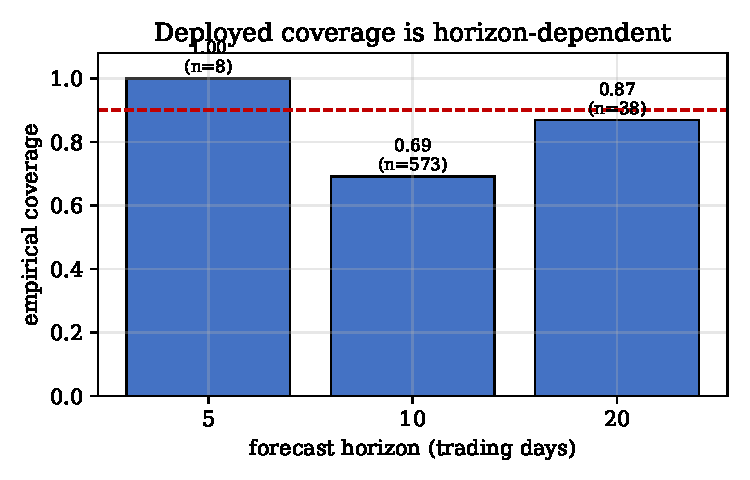
\includegraphics[width=0.82\linewidth]{fig_coverage_horizon.pdf}
\caption{Empirical coverage by forecast horizon (dashed line: nominal $0.90$). The
ten-day stratum, which holds $573$ of $619$ forecasts, carries the shortfall; the
sparse longer horizons are mildly conservative.}
\label{fig:horizon}
\end{figure}

\subsection{Width does not explain miscoverage}
A natural hypothesis is that the narrow intervals are the uncovered ones --- that
coverage simply tracks width. It does not. Splitting forecasts into normalized-width
quartiles yields coverage $0.72, 0.68, 0.69, 0.73$ from sharpest to widest
(Figure~\ref{fig:cond}a). Coverage is flat in width: the widest quartile is no better
covered than the sharpest. Whatever is breaking the intervals is not captured by how
wide they happen to be.

\subsection{The confidence--coverage inversion}
The covariate that \emph{does} explain miscoverage is the magnitude of the point
forecast. Partitioning forecasts into tertiles of $|f_t|$ gives coverage
$0.957$ (low, mean $|f|=0.6\%$), $0.689$ (mid, $1.9\%$), and $0.471$ (high,
$4.3\%$): coverage falls monotonically and steeply as the model becomes more
opinionated (Figure~\ref{fig:cond}b). On the third of forecasts where the model
predicts the largest moves, fewer than half of the realized prices land inside the
$90\%$ band. The system is least reliable exactly where it is most confident.

\begin{figure}[t]
\centering
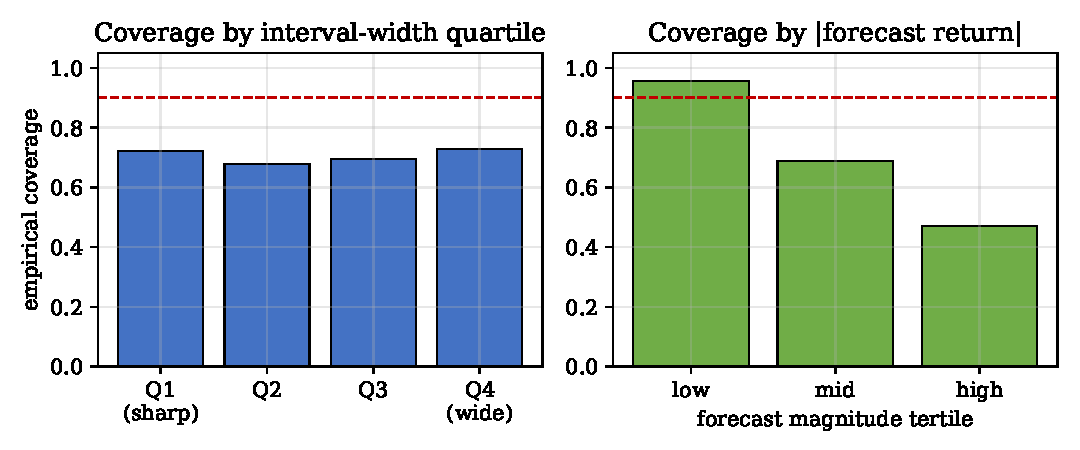
\includegraphics[width=\linewidth]{fig_conditional_coverage.pdf}
\caption{Conditional coverage. \textbf{(a)} Coverage is flat across interval-width
quartiles. \textbf{(b)} Coverage collapses with forecast magnitude, from $95.7\%$
on the least opinionated third of forecasts to $47.1\%$ on the most opinionated
third. Dashed line: nominal $0.90$.}
\label{fig:cond}
\end{figure}

The mechanism is that the interval generator does not widen enough for confident
forecasts. The correlation between normalized width $w_t$ and forecast magnitude
$|f_t|$ is only $0.27$; the median width grows from $0.107$ on the low-magnitude
tertile to just $0.129$ on the high-magnitude tertile --- a $20\%$ increase in width
to accompany a roughly seven-fold increase in forecast magnitude. An aggressive
forecast is thus quoted with a band scarcely wider than a timid one. Because the point
forecasts carry no directional edge (the realized sign matches the forecast sign only
$45.7\%$ of the time, below a coin), large forecasts are followed by reversion as often
as not, and a band that failed to widen is blown through. The inversion is the
interval-level shadow of an
over-extrapolating point forecast.

A small but telling corollary: $94.0\%$ of the intervals \emph{straddle the anchor}
price, i.e.\ they do not commit to a direction at the $90\%$ level. The system already
``knows,'' through the width of its bands, that it usually should not commit. The
failure is concentrated in the minority of cases where it does commit --- and there it
under-covers most.

\subsection{Heterogeneity across instruments}
Per-instrument coverage (names with $\ge 10$ resolved forecasts) ranges from $0.46$
to $0.94$, mean $0.68$. The dispersion is wide enough that a single marginal number
hides instruments whose intervals are badly broken and others that are nearly honest.
We return to instrument conditioning, alongside magnitude conditioning, when we ask
what the data can support in Section~\ref{sec:results}.

% =============================================================================
\section{A Minimal Conformal Recalibration}\label{sec:method}
% =============================================================================
\subsection{Multiplicative width recalibration}
We correction the bands with the smallest instrument that the diagnosis licenses: a scalar
multiplicative rescaling of each interval's half-width about its own center. For a
factor $\lambda>0$ the recalibrated interval is
\begin{equation}
[\,c_t - \lambda\,\mathit{hw}_t,\; c_t + \lambda\,\mathit{hw}_t\,].
\end{equation}
Define the symmetric nonconformity score
$\rho_t = |P_{t+h}-c_t| / \mathit{hw}_t$, the number of half-widths by which the
realized price misses the center. The recalibrated interval covers iff
$\rho_t \le \lambda$, so empirical coverage at multiplier $\lambda$ is exactly the
empirical CDF of $\rho$ evaluated at $\lambda$:
\begin{equation}
\widehat{C}(\lambda) = \tfrac1n\textstyle\sum_t \mathbb{1}\{\rho_t \le \lambda\}.
\end{equation}
This makes the entire coverage--width trade-off a single monotone curve
(Figure~\ref{fig:lambda}), and the choice of $\lambda$ a one-dimensional conformal
calibration.

\begin{definition}[Split-conformal multiplier]
Given a calibration set $\mathcal{C}$ of size $m$, the conformal multiplier at level
$1-\alpha$ is the $\lceil (m+1)(1-\alpha)\rceil$-th smallest value of
$\{\rho_t : t\in\mathcal{C}\}$. Applied to an exchangeable test forecast, it yields
marginal coverage at least $1-\alpha$ \cite{vovk2005,romano2019}.
\end{definition}

\subsection{Global versus magnitude-conditional}
The diagnosis suggests conditioning $\lambda$ on forecast magnitude. We therefore
compare two estimators, both fitted only on the calibration window:
\begin{itemize}[leftmargin=1.4em,itemsep=1pt]
\item \textbf{Global:} one multiplier $\lambda^\star$ from all calibration scores.
\item \textbf{Magnitude-conditional:} a separate multiplier $\lambda^\star_b$ for each
tertile $b$ of $|f_t|$, applied to test forecasts according to their own magnitude.
\end{itemize}
We deliberately do \emph{not} fit per-horizon or per-instrument multipliers on this
sample: with most strata holding only tens of forecasts, a stratified multiplier is an
extreme order statistic of a tiny set and would overfit. The same caution governs how
we read the magnitude-conditional result.

\subsection{Protocol and metrics}
Forecasts are ordered by issue time and split $60/40$ into a past calibration window
($m=371$) and a future test window ($248$); multipliers are fit on the former and all
coverage and sharpness numbers are reported on the latter, so the evaluation is
strictly walk-forward. We report empirical coverage, median normalized width
(sharpness), and the normalized interval (Winkler) score
\begin{equation}
S_\alpha = \frac{(H-L) + \frac{2}{\alpha}(L-y)\mathbb{1}\{y<L\}
+ \frac{2}{\alpha}(y-H)\mathbb{1}\{y>H\}}{P},
\end{equation}
which is a proper scoring rule (lower is better) rewarding sharpness subject to
coverage \cite{winkler1972,gneiting2007}. We summarize conditional calibration by the
mean absolute coverage gap across magnitude tertiles,
$\overline{\Delta}=\tfrac13\sum_b |\widehat{C}_b - 0.90|$.

% =============================================================================
\section{Results}\label{sec:results}
% =============================================================================
\subsection{Global recalibration restores coverage}
On the held-out test window the raw intervals cover $0.718$. The global conformal
multiplier estimated on the calibration window is $\lambda^\star = 1.54$: the bands
must be widened by about half to keep their promise. Applied walk-forward it lifts
test coverage to $0.944$ and lowers the mean interval score from $0.218$ to $0.185$
(Table~\ref{tab:recal}). The improvement in a \emph{proper} score is the important
part: coverage is restored not by indiscriminate widening (which a proper score would
penalize through the width term) but by a correction that the score certifies as a
better forecast. Figure~\ref{fig:lambda} shows the full coverage--$\lambda$ curve; the
deployed system sits at $\lambda=1$ with $0.706$ coverage, and the nominal target is
reached at $\lambda^\star$.

\begin{figure}[t]
\centering
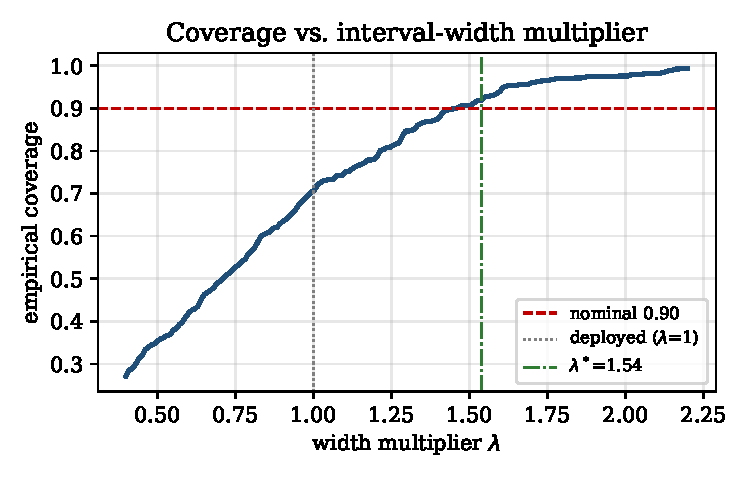
\includegraphics[width=0.82\linewidth]{fig_coverage_lambda.pdf}
\caption{Coverage as a function of the width multiplier $\lambda$ (whole sample).
The deployed bands ($\lambda=1$) cover $70.6\%$; the conformal multiplier
$\lambda^\star=1.54$ reaches the nominal $0.90$. The curve is the empirical CDF of the
nonconformity score $\rho$.}
\label{fig:lambda}
\end{figure}

\begin{table}[t]
\centering
\caption{Walk-forward recalibration on the held-out test window ($248$ forecasts).
Coverage target $0.90$; interval score lower is better; $\overline{\Delta}$ is the
mean absolute coverage gap across magnitude tertiles.}
\label{tab:recal}
\small
\begin{tabular}{lcccc}
\toprule
Method & Coverage & Median $w$ & Int.\ score & $\overline{\Delta}$ \\
\midrule
Deployed ($\lambda{=}1$) & $0.718$ & $0.109$ & $0.218$ & $0.156$ \\
Global ($\lambda^\star{=}1.54$) & $0.944$ & $0.168$ & $0.185$ & $0.071$ \\
Magnitude-conditional & $0.980$ & $0.195$ & --- & $0.073$ \\
\bottomrule
\end{tabular}
\end{table}

\subsection{An honest negative result on conditioning}
The magnitude-conditional fit recovers exactly the corrections the diagnosis predicts:
its tertile multipliers are $\lambda^\star_{\text{low}}=0.89$,
$\lambda^\star_{\text{mid}}=1.40$, $\lambda^\star_{\text{high}}=2.02$. It \emph{shrinks}
the timid intervals (which were over-covering) and roughly \emph{doubles} the confident
ones (which were badly under-covering). This is the structurally correct behavior, and
it is reassuring that an unsupervised conformal fit discovers it. Yet on the held-out
window it does not beat the global fix on the trade-off that matters: the mean tertile
coverage gap is $\overline{\Delta}=0.073$ for the conditional fit versus $0.071$ for
the global one, while the conditional fit's median width is larger
(Figure~\ref{fig:recal}, Table~\ref{tab:recal}). The reason is sample size: the global
multiplier already drags the worst (high-magnitude) tertile from $0.58$ to $0.91$ on
the test split, and the conditional fit's high-magnitude multiplier ($\lambda=2.02$)
is an order statistic of only a few dozen calibration forecasts, so it overshoots to
$0.99$ rather than landing on $0.90$.

\begin{figure}[t]
\centering
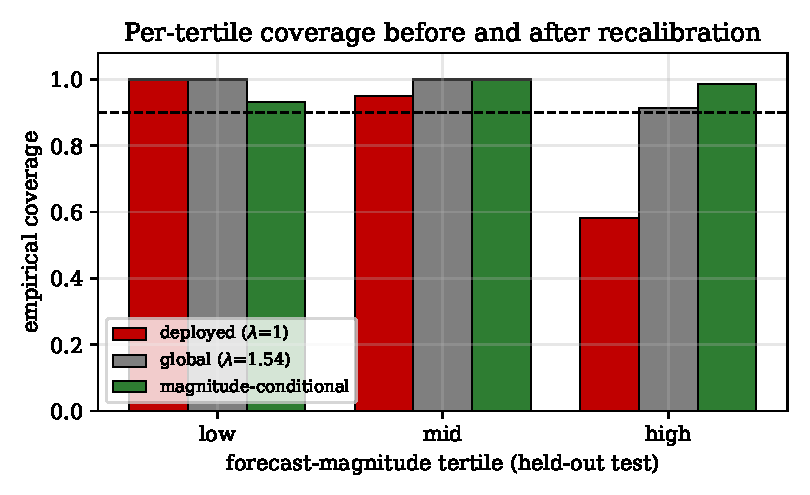
\includegraphics[width=0.82\linewidth]{fig_magnitude_recal.pdf}
\caption{Per-magnitude-tertile coverage on the held-out test window before and after
recalibration. The deployed bands under-cover the confident (high-magnitude) tertile
at $0.58$; the global fix lifts it to $0.91$; the magnitude-conditional fit applies
the correctly-signed but noisier corrections and overshoots. Dashed line: nominal
$0.90$.}
\label{fig:recal}
\end{figure}

We therefore decline to claim the conditional method on this data, and we state the
criterion for adopting it: magnitude conditioning should be deployed once the
calibration window contains enough high-magnitude resolved forecasts that the
$0.90$-quantile of their nonconformity scores is stable --- concretely, when the
high-magnitude calibration count is large enough that bootstrap resampling of
$\lambda^\star_{\text{high}}$ has a coefficient of variation below, say, $0.1$. On the
present sample it is far above that. The restraint is itself a result: in a thin
deployment, a single global recalibration captures most of the recoverable coverage,
and conditioning is a structure to grow into, not a knob to turn now.

\subsection{Stability over the deployment window}
Figure~\ref{fig:temporal} tracks weekly coverage across the deployment. The deployed
bands hover well below nominal throughout, with no week reaching $0.90$, while the
globally recalibrated bands sit around nominal across weeks. The miscoverage is thus a
persistent property of the system, not an artifact of one turbulent week --- which is
what licenses a static multiplicative correction rather than a reactive one. (How quickly
such a multiplier should be refreshed as the regime drifts is a separate question,
addressed by recalibration-cadence analyses and outside our scope here.)

\begin{figure}[t]
\centering
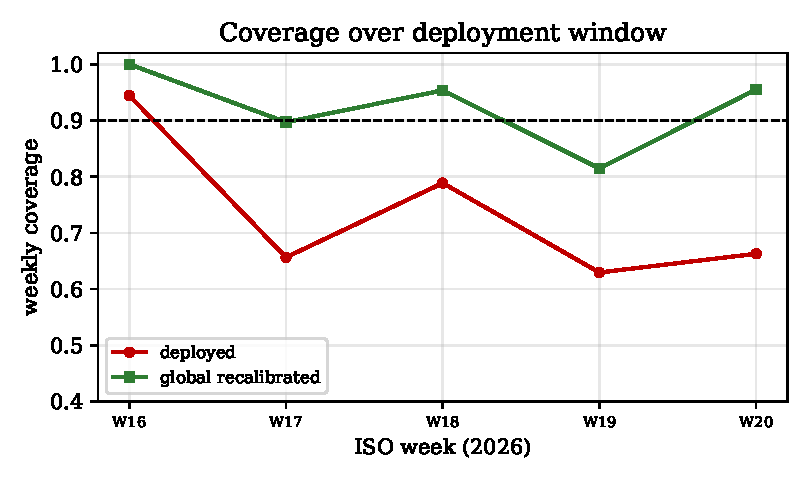
\includegraphics[width=0.86\linewidth]{fig_temporal_coverage.pdf}
\caption{Weekly empirical coverage over the deployment window. Deployed intervals
(red) never reach nominal; globally recalibrated intervals (green) track $0.90$.}
\label{fig:temporal}
\end{figure}

% =============================================================================
\section{Discussion}\label{sec:discussion}
% =============================================================================
\textbf{Why confidence and coverage invert.} The inversion is not a bug peculiar to
one system; it is what one should expect whenever a point forecaster operating near
the efficiency limit emits intervals whose width is decoupled from its own
conviction. Near efficiency, large predicted moves are not more likely to be realized;
if anything they revert. An interval that widens with horizon and volatility but not
with the forecast's own magnitude will therefore cover the timid forecasts (whose
small predicted moves sit comfortably inside a horizon-scaled band) and fail the
confident ones (whose large predicted moves push the center away from where the price
actually goes, while the band stays put). The remedy is to tie interval width to the
quantity that actually predicts miss size --- here, forecast magnitude --- rather than to
proxies like width or horizon that do not. This is a design principle, not a
parameter: \emph{an interval should widen in step with the boldness of the point it
surrounds.}

\textbf{Coverage is necessary, not sufficient.} We have been careful to evaluate the
correction with a proper score, because coverage alone is a corruptible target: any band
can be made to cover by inflating it. The interval-score improvement
($0.218\to0.185$) certifies that the conformal widening buys coverage at an honest
price in sharpness. Practitioners studying their own systems should report both, and
should treat a coverage fix that worsens a proper score as a warning, not a success.

\textbf{The point is not the product; the interval is.} The forecasts studied here
carry no directional edge --- realized sign matches forecast sign $45.7\%$ of the time,
below a coin. It would be easy to read this as a failure of the system. We read it
differently: in a near-efficient market the honest deliverable is calibrated
uncertainty, and a system that abstains from directional commitment on $94\%$ of cases
(its bands straddle the anchor) and quotes a trustworthy band on the rest is behaving
correctly --- \emph{provided the band is trustworthy.} That proviso is the whole point of
this paper, and it is exactly the property that was broken and is now corrected.

% =============================================================================
\section{Threats to Validity and Reproducibility}\label{sec:threats}
% =============================================================================
\textbf{Sample scope.} The analysis covers six instruments over about eight weeks in a
single market regime. The numbers characterize this deployment, not equities at large;
coverage, the multiplier $\lambda^\star$, and the magnitude structure could differ in
another regime. We have therefore framed every quantitative claim as a property of the
ledger and have avoided extrapolation. The qualitative result --- that miscoverage is
indexed by forecast magnitude, not width --- is mechanistic and we expect it to recur
wherever interval width is decoupled from forecast conviction, but that is a
hypothesis for replication, not a proven generalization.

\textbf{Exchangeability.} The split-conformal guarantee assumes exchangeability
between calibration and test forecasts. Markets drift, so the assumption is
approximate; this is precisely why we report walk-forward coverage on a future window
rather than relying on the in-sample guarantee, and why the temporal-stability check
matters.

\textbf{Reproducibility.} The analysis is a deterministic function of an immutable
ledger. Given the ledger, every figure and table in this paper is regenerated by a
single script that recomputes coverage, the nonconformity scores, the conformal
multipliers under the fixed $60/40$ time split, and the interval scores. No randomness
enters except the fixed split point, which is determined by issue-time ordering. The
nonconformity score, the conformal quantile rule, and the interval score are stated in
closed form in Sections~\ref{sec:method}. We regard the write-once, point-in-time
ledger as the reusable artifact: any team that records forecasts this way can run the
same analysis on its own system.

% =============================================================================
\section{Conclusion}\label{sec:conclusion}
% =============================================================================
We studied the prediction intervals of a deployed equity forecaster against an
append-only, leakage-free ledger and found them overconfident ($70.6\%$ coverage for a
nominal $90\%$ band). The substantive finding is structural: miscoverage is governed
not by interval width --- coverage is flat across width quartiles --- but by the magnitude
of the point forecast, collapsing from $95.7\%$ to $47.1\%$ as the model grows more
opinionated, because the bands fail to widen for confident forecasts. A one-parameter
split-conformal width recalibration estimated on past forecasts restores coverage to
$94.4\%$ walk-forward and improves a proper interval score, while a
magnitude-conditional refinement recovers the correct corrections but is not yet
justified by the sample. The practical message is compact: in a near-efficient regime,
\emph{confidence is not coverage}, and an interval keeps its promise only if its width
scales with the boldness of the point it surrounds. The evaluation procedure --- a write-once
ledger, a magnitude-indexed coverage diagnosis, and a conformal correction scored by a
proper rule --- transfers to any deployed probabilistic forecaster.

% =============================================================================
\section*{Acknowledgements}
% =============================================================================
\textbf{Use of AI tools.} Generative AI assistance (a large language model) was used
for language editing and for drafting and refactoring the analysis and
figure-generation scripts. All quantitative results were computed by the authors'
deterministic code directly from the deployment ledger and were verified by the
authors; no numerical result, table, or figure was produced by a language model. The
authors take full responsibility for the content.

% =============================================================================
\begin{thebibliography}{99}
\setlength{\itemsep}{1pt}

\bibitem{guo2017} C.~Guo, G.~Pleiss, Y.~Sun, and K.~Q. Weinberger, ``On calibration of
modern neural networks,'' in \emph{Proc.\ 34th Int.\ Conf.\ Machine Learning (ICML)},
2017, pp.\ 1321--1330.

\bibitem{ovadia2019} Y.~Ovadia \emph{et al.}, ``Can you trust your model's uncertainty?
Evaluating predictive uncertainty under dataset shift,'' in \emph{Advances in Neural
Information Processing Systems (NeurIPS)}, vol.\ 32, 2019.

\bibitem{lakshminarayanan2017} B.~Lakshminarayanan, A.~Pritzel, and C.~Blundell,
``Simple and scalable predictive uncertainty estimation using deep ensembles,'' in
\emph{Advances in Neural Information Processing Systems (NeurIPS)}, vol.\ 30, 2017.

\bibitem{platt1999} J.~Platt, ``Probabilistic outputs for support vector machines and
comparisons to regularized likelihood methods,'' \emph{Advances in Large Margin
Classifiers}, vol.\ 10, no.\ 3, pp.\ 61--74, 1999.

\bibitem{zadrozny2002} B.~Zadrozny and C.~Elkan, ``Transforming classifier scores into
accurate multiclass probability estimates,'' in \emph{Proc.\ 8th ACM SIGKDD Int.\ Conf.\
Knowledge Discovery and Data Mining}, 2002, pp.\ 694--699.

\bibitem{naeini2015} M.~P. Naeini, G.~Cooper, and M.~Hauskrecht, ``Obtaining well
calibrated probabilities using Bayesian binning,'' in \emph{Proc.\ AAAI Conf.\
Artificial Intelligence}, vol.\ 29, 2015.

\bibitem{brier1950} G.~W. Brier, ``Verification of forecasts expressed in terms of
probability,'' \emph{Monthly Weather Review}, vol.\ 78, no.\ 1, pp.\ 1--3, 1950.

\bibitem{vovk2005} V.~Vovk, A.~Gammerman, and G.~Shafer, \emph{Algorithmic Learning in
a Random World}. New York, NY, USA: Springer, 2005.

\bibitem{shafer2008} G.~Shafer and V.~Vovk, ``A tutorial on conformal prediction,''
\emph{Journal of Machine Learning Research}, vol.\ 9, pp.\ 371--421, 2008.

\bibitem{angelopoulos2023} A.~N. Angelopoulos and S.~Bates, ``Conformal prediction: a
gentle introduction,'' \emph{Foundations and Trends in Machine Learning}, vol.\ 16,
no.\ 4, pp.\ 494--591, 2023.

\bibitem{romano2019} Y.~Romano, E.~Patterson, and E.~Cand\`es, ``Conformalized quantile
regression,'' in \emph{Advances in Neural Information Processing Systems (NeurIPS)},
vol.\ 32, 2019.

\bibitem{gibbs2021} I.~Gibbs and E.~Cand\`es, ``Adaptive conformal inference under
distribution shift,'' in \emph{Advances in Neural Information Processing Systems
(NeurIPS)}, vol.\ 34, 2021, pp.\ 1660--1672.

\bibitem{xu2023} C.~Xu and Y.~Xie, ``Conformal prediction for time series,'' \emph{IEEE
Transactions on Pattern Analysis and Machine Intelligence}, vol.\ 45, no.\ 10,
pp.\ 11575--11587, 2023.

\bibitem{gneiting2007} T.~Gneiting and A.~E. Raftery, ``Strictly proper scoring rules,
prediction, and estimation,'' \emph{Journal of the American Statistical Association},
vol.\ 102, no.\ 477, pp.\ 359--378, 2007.

\bibitem{gneiting2007probabilistic} T.~Gneiting, F.~Balabdaoui, and A.~E. Raftery,
``Probabilistic forecasts, calibration and sharpness,'' \emph{Journal of the Royal
Statistical Society: Series B}, vol.\ 69, no.\ 2, pp.\ 243--268, 2007.

\bibitem{winkler1972} R.~L. Winkler, ``A decision-theoretic approach to interval
estimation,'' \emph{Journal of the American Statistical Association}, vol.\ 67,
no.\ 337, pp.\ 187--191, 1972.

\bibitem{bailey2014} D.~H. Bailey, J.~Borwein, M.~L\'opez de Prado, and Q.~J. Zhu,
``Pseudo-mathematics and financial charlatanism: the effects of backtest overfitting
on out-of-sample performance,'' \emph{Notices of the American Mathematical Society},
vol.\ 61, no.\ 5, pp.\ 458--471, 2014.

\bibitem{harvey2016} C.~R. Harvey, Y.~Liu, and H.~Zhu, ``$\ldots$ and the
cross-section of expected returns,'' \emph{Review of Financial Studies}, vol.\ 29,
no.\ 1, pp.\ 5--68, 2016.

\bibitem{lopez2018} M.~L\'opez de Prado, \emph{Advances in Financial Machine
Learning}. Hoboken, NJ, USA: Wiley, 2018.

\bibitem{fama1970} E.~F. Fama, ``Efficient capital markets: a review of theory and
empirical work,'' \emph{Journal of Finance}, vol.\ 25, no.\ 2, pp.\ 383--417, 1970.

\bibitem{malkiel2003} B.~G. Malkiel, ``The efficient market hypothesis and its
critics,'' \emph{Journal of Economic Perspectives}, vol.\ 17, no.\ 1, pp.\ 59--82,
2003.

\bibitem{welch2008} I.~Welch and A.~Goyal, ``A comprehensive look at the empirical
performance of equity premium prediction,'' \emph{Review of Financial Studies},
vol.\ 21, no.\ 4, pp.\ 1455--1508, 2008.

\bibitem{fischer2018} T.~Fischer and C.~Krauss, ``Deep learning with long short-term
memory networks for financial market predictions,'' \emph{European Journal of
Operational Research}, vol.\ 270, no.\ 2, pp.\ 654--669, 2018.

\bibitem{gu2020} S.~Gu, B.~Kelly, and D.~Xiu, ``Empirical asset pricing via machine
learning,'' \emph{Review of Financial Studies}, vol.\ 33, no.\ 5, pp.\ 2223--2273,
2020.

\end{thebibliography}

\end{document}
